\documentclass[12pt]{article}

\usepackage[letterpaper,margin=1in]{geometry}

\setlength{\parindent}{0pt}

\usepackage{amssymb}
\usepackage{amsmath}

\usepackage{multicol}

\usepackage{tikz}

\newcommand{\headerText}{
  MA 238 | Fall 2018 | Dr. Clontz
}

\usepackage{fancyhdr}
\pagestyle{fancy}
\renewcommand{\headrulewidth}{0pt}% Default \headrulewidth is 0.4pt
\renewcommand{\footrulewidth}{0pt}% Default \footrulewidth is 0pt
\chead{\footnotesize\bf\headerText}
\cfoot{}

\newcommand{\csch}{\operatorname{csch}}
\newcommand{\sech}{\operatorname{sech}}

\newcommand{\issuesMark}{{\fontencoding{U}\fontfamily{futs}\selectfont\char 66\relax}}





\begin{document}


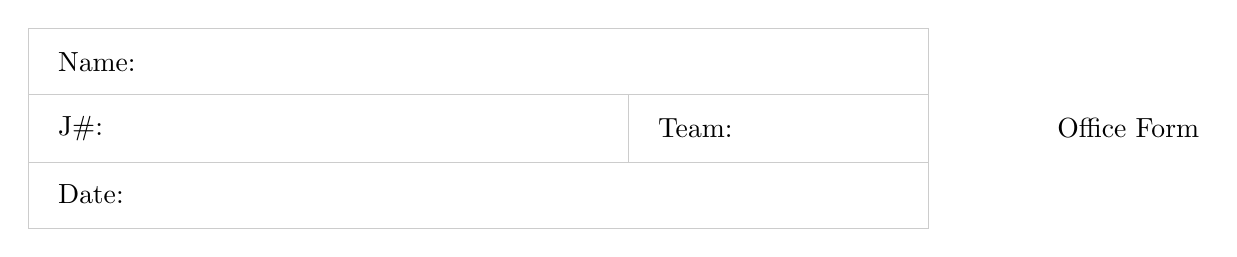
\begin{tikzpicture}[x=1in,y=1in]
  \draw[color=black!20] (0,0) rectangle (4.5,1);
  \draw[color=black!20] (0,0.67) -- (4.5,0.67);
  \draw[color=black!20] (3,0.33) -- (3,0.67);
  \draw[color=black!20] (0,0.33) -- (4.5,0.33);

  \node[anchor=west] at (0.1,0.83) {Name:};
  \node[anchor=west] at (0.1,0.5) {J\#:};
  \node[anchor=west] at (3.1,0.5) {Team:};
  \node[anchor=west] at (0.1,0.17) {Date:};

  \node at (5.5,0.5) {Office Form}; 
\end{tikzpicture}

\vspace{1em}

\begin{tikzpicture}[x=1in,y=1in]
  \draw[color=black!50] (0,0) rectangle (6.4,1);
  \draw[color=black!50] (1,0) -- (1,1);
  \draw[color=black!50] (5.4,0) -- (5.4,1);

  \node[anchor=north west,color=black!70] at (0,0.95) {\footnotesize Standard:};
  \node[anchor=north west,color=black!70] at (5.4,0.95) {\footnotesize Mark:};
\end{tikzpicture}


\renewcommand\labelitemi{\(\square\)}
Mark all that apply.
\begin{itemize}
  \item \textbf{I have attempted this standard before.}
        You have received a mark of \issuesMark{} or better on a previous Mastery Quiz
        for this standard.
  \item \textbf{I am active in the course.}
        You have satisfied all the criteria outlined on the syllabus to be
        considered an Active student.
  \item \textbf{This standard will not be included on a Mastery Quiz today.}
        Two mastery checkmarks cannot be earned for the same standard on the same day.
  \item \textbf{This is my first, second, third, or fourth Office Form for the week.}
        You may not submit more than fourth Office Forms each week.
  \item \textbf{I have completed at least two old quiz exercises
        relevant to this standard.}
        You have written these complete solutions on this form, or attached the solutions
        to this form. Both exercises must have been assigned to you personally
        on a previous mastery quiz.
\end{itemize}

If you meet all these requirements,
bring this form to the instructor's office hours. 
If the attached exercises have been worked correctly, you will be given
a new exercise to complete in the office, which will be marked immediately for credit.
\newpage


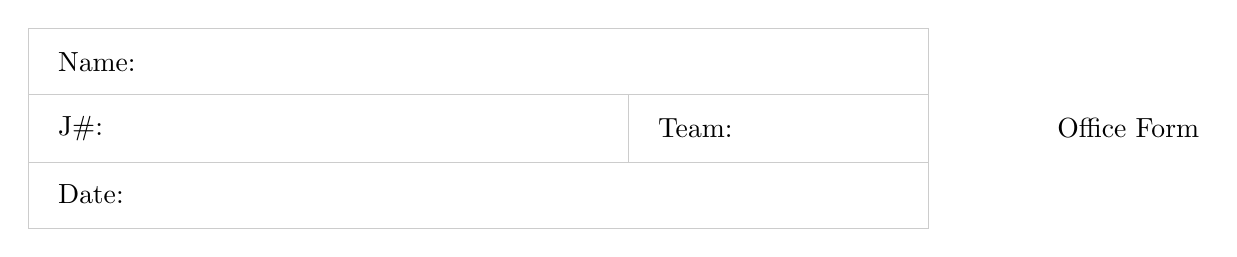
\begin{tikzpicture}[x=1in,y=1in]
  \draw[color=black!20] (0,0) rectangle (4.5,1);
  \draw[color=black!20] (0,0.67) -- (4.5,0.67);
  \draw[color=black!20] (3,0.33) -- (3,0.67);
  \draw[color=black!20] (0,0.33) -- (4.5,0.33);

  \node[anchor=west] at (0.1,0.83) {Name:};
  \node[anchor=west] at (0.1,0.5) {J\#:};
  \node[anchor=west] at (3.1,0.5) {Team:};
  \node[anchor=west] at (0.1,0.17) {Date:};

  \node at (5.5,0.5) {Office Form}; 
\end{tikzpicture}

\vspace{1em}

\begin{tikzpicture}[x=1in,y=1in]
  \draw[color=black!50] (0,0) rectangle (6.4,1);
  \draw[color=black!50] (1,0) -- (1,1);
  \draw[color=black!50] (5.4,0) -- (5.4,1);

  \node[anchor=north west,color=black!70] at (0,0.95) {\footnotesize Standard:};
  \node[anchor=north west,color=black!70] at (5.4,0.95) {\footnotesize Mark:};
\end{tikzpicture}


\renewcommand\labelitemi{\(\square\)}
Mark all that apply.
\begin{itemize}
  \item \textbf{I have attempted this standard before.}
        You have received a mark of \issuesMark{} or better on a previous Mastery Quiz
        for this standard.
  \item \textbf{I am active in the course.}
        You have satisfied all the criteria outlined on the syllabus to be
        considered an Active student.
  \item \textbf{This standard will not be included on a Mastery Quiz today.}
        Two mastery checkmarks cannot be earned for the same standard on the same day.
  \item \textbf{I have previously submitted no more than two Office Forms this week.}
        You may not submit more than three Office Forms each week.
  \item \textbf{I have completed at least two old quiz exercises
        relevant to this standard.}
        You have written these complete solutions on this form, or attached the solutions
        to this form. Both exercises must have been assigned to you personally
        on a previous mastery quiz.
\end{itemize}

If you meet all these requirements,
bring this form to the instructor's office hours. 
If the attached exercises have been worked correctly, you will be given
a new exercise to complete in the office, which will be marked immediately for credit.
\end{document}
